\section{Eigenanalysis, Singular Value Decomposition of Data Matrices}
\label{sec:datasvd}

Singular Value Decomposition (SVD) is a matrix decomposition of the form $\mathbf{A}=\mathbf{U}\Sigma\mathbf{V}^T$, where $\mathbf{U}$ and $\mathbf{V}$ are both unitary (cf. section \ref{sec:svd}). The decomposition always exists for a general complex matrix $\mathbf{A}\in\mathbb{C}^{m\times n}$. 
\\

If $\mathbf{X}\in\mathbb{R}^{N\times p}$ is a data matrix with $N$ samples in the rows and $p$ features in the columns, then SVD allows for the decomposition of the data into $p$ linearly independent components, ranked by their explained variance (i.e. their strength in the dataset). The basis of the decomposition turns out the same as for PCA (cf. section \ref{sec:pca}) except that it is arrived at slightly differently, because PCA involves diagonalizing the covariance matrix. The decomposition of the dataset can be understood as follows. In the SVD of the data matrix: 

\begin{equation}
\mathbf{X} = \mathbf{U}\mathbf{\Sigma}\mathbf{V}^T
\end{equation}

The individual rows of $\mathbf{X}$, i.e. the individual data points, are expressed as:

\begin{equation}
\mathbf{x}^T_i = \sum_{j=1}^p u_{i,j}\sigma_j\mathbf{v}_j^T
\end{equation}

Where $\mathbf{x}_i$ is the $i$th data point. Hence the right singular vectors $\mathbf{v}_i$ are the normalized basis vectors, and the columns of $\mathbf{U}$ give the coefficients the basis expansion, together with the singular values $\sigma_i$, which give a measure of the global strength of the corresponding basis vector. 

SVD is scalable to very large datasets and finds many applications in the wild, including page rank, facial recognition, recommendation algorithms etc. 


% eigenfaces
\subsection{Example: Eigenfaces and Facial Recognition}
One famous result are the so-called eigenfaces. The data matrix $\mathbf{X}\in\mathbb{R}^{N\times p}$ consists of $N$ pictures of faces that each have $p$ pixels. The right singular eigenvectors yield $p$ eigenfaces in terms of which any of the $N$ pictures can be expressed. 

Below are the first eigenfaces extracted from the "Labeled Faces in the Wild" dataset, which includes 13233 portraits with 62x47=2914 pixels each. Running SVD on the data matrix $\mathbf{X} \in \mathbb{R}^{13233\times 2914}$ yields the eigenfaces shown in Figure \ref{fig:svd_eigenfaces}.

\begin{figure}
\centering
    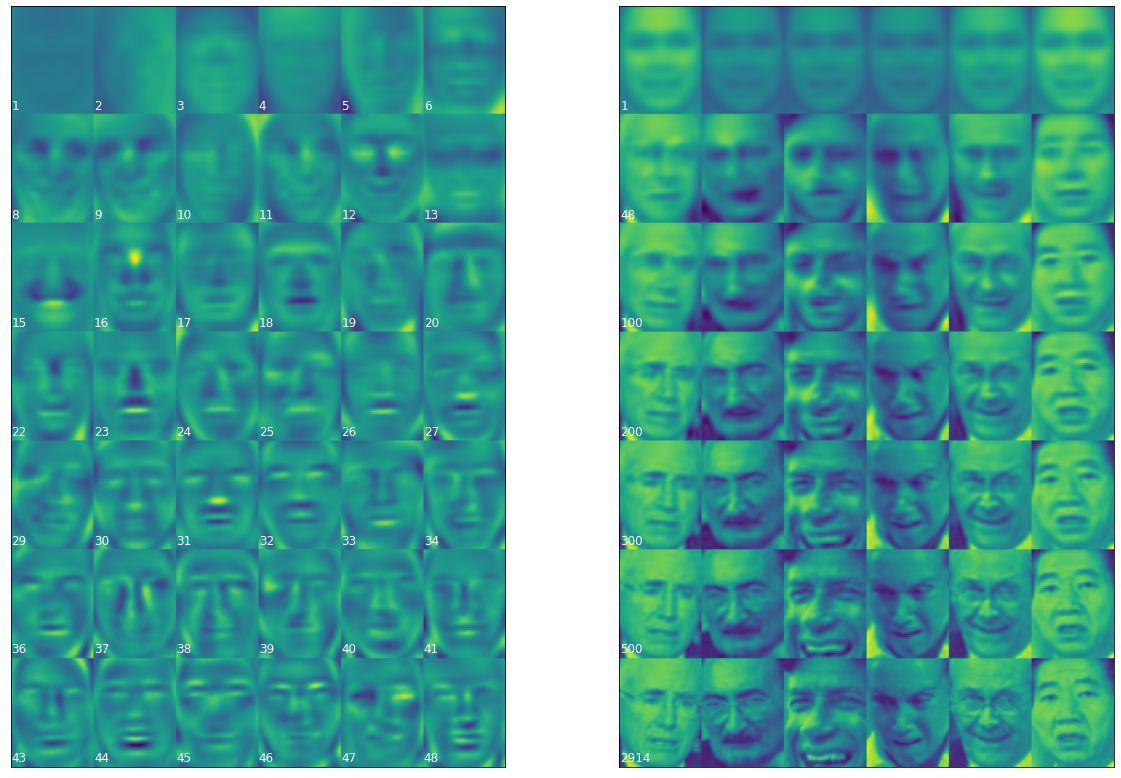
\includegraphics[width=\textwidth]{svd_eigenfaces.png}
    \caption{Left: The first 48 eigenfaces. The colorscale is consistent across the images. As can be expected, the eigenfaces seem to have an ordering from more general features, that are highly prevalent in the dataset, towards more specific features. Right: Five sample portraits from the dataset approximated using different numbers of eigenvectors. 2914 corresponds to the original image, which had 2914 pixels (degrees of freedom).}
    \label{fig:svd_eigenfaces}
\end{figure}

Facial recognition may be performed by projecting a new face into the space of eigenfaces and some form of matching to the coefficients of a known subject. This could be simply the euclidean distance, or it could be a classifier. In case of a classifier, the dimensionality reduction that is enabled by approximating images with a smaller set of eigenvectors may be critical to making the problem tractable by overcoming the curse of dimensionality.


% eigenbasis 
\subsection{Constructing A Consistently Oriented Eigenbasis}
	
As discussed in section \ref{sec:svd}, the sign of the basis vectors can be flipped without affecting the validity of the singular value decomposition. That means that if the SVD is performed repeatedly on a slowly evolving system, the derived eigenbasis of the system can abruptly change, from, for example, a left-handed to a right-handed coordinate system. Hence there is a need to find a way to consistently orient the basis of eigenvectors. 

Heuristic techniques can work by taking the dot product between the singular vectors derived for two separate SVDs, and flipping them whenever the dot product is negative. A more rigorous technique was derived by \citeasnoun{damask2019consistently}. \possessivecite{damask2019consistently} technique relies on constructing the sequence of reflection and rotation operations necessary to transform a constituent basis into the derived eigenbasis. The gradual transformation begins with the singular vector with the largest singular value, because it has the greatest numerical certainty. 

Once consistently oriented, directional statistics (cf. section \ref{sec:directionalstats}) can be applied to analyze the evolution of the eigensystem over different measurements. 

In general, singular vectors are only labeled by their corresponding singular value (assuming no degeneracy). Rank order changes require attaching an additional label to the eigenvectors.

\begin{figure}
\centering
    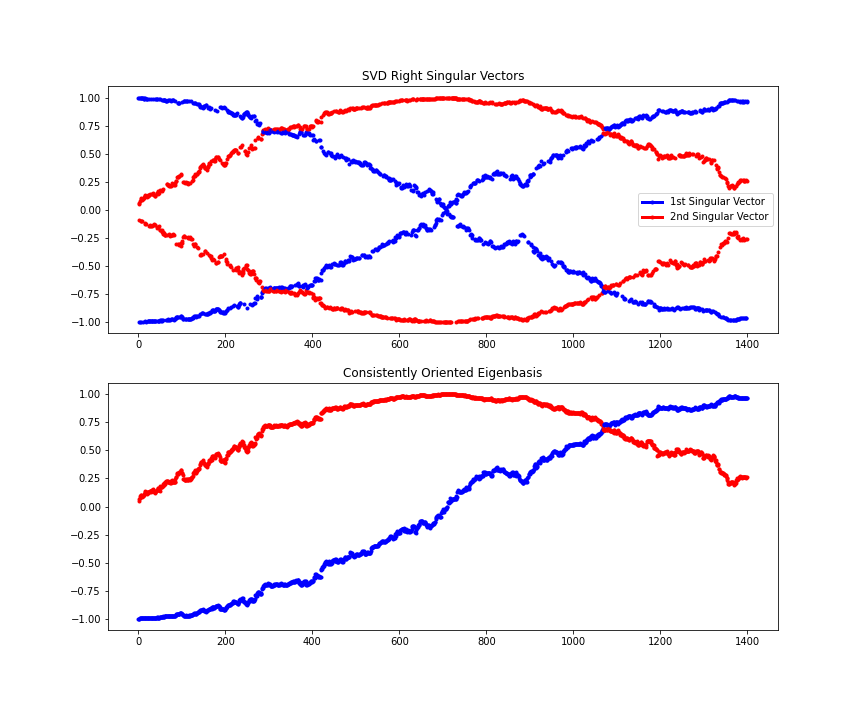
\includegraphics[width=\textwidth]{svd_consistently_oriented.png}
    \caption{Right singular vectors extracted using SVD, showing sign flips (top) and with a consistently oriented basis (bottom). The underlying data is a bivariate gaussian with principal axes undergoing a 180 degree rotation. With the consistently oriented basis, the singular vectors trace out a one-to-one trajectory that can be analyzed.}
    \label{fig:svd_consistently_oriented}
\end{figure}
